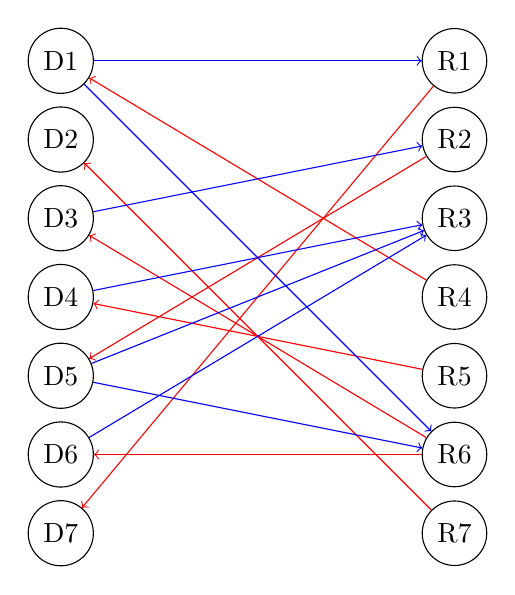
\begin{tikzpicture}
\node at (0,3) [draw,shape = circle](D1){D1};
\node at (0,2) [draw,shape = circle](D2){D2};
\node at (0,1) [draw,shape = circle](D3){D3};
\node at (0,0) [draw,shape = circle](D4){D4};
\node at (0,-1) [draw,shape = circle](D5){D5};
\node at (0,-2) [draw,shape = circle](D6){D6};
\node at (0,-3) [draw,shape = circle](D7){D7};
\node at (5,3) [draw,shape = circle](R1){R1};
\node at (5,2) [draw,shape = circle](R2){R2};
\node at (5,1) [draw,shape = circle](R3){R3};
\node at (5,0) [draw,shape = circle](R4){R4};
\node at (5,-1) [draw,shape = circle](R5){R5};
\node at (5,-2) [draw,shape = circle](R6){R6};
\node at (5,-3) [draw,shape = circle](R7){R7};
\draw[<-, color = red] (D1) -- (R4);
\draw[<-, color = red] (D2) -- (R7);
\draw[<-, color = red] (D3) -- (R6);
\draw[<-, color = red] (D4) -- (R5);
\draw[<-, color = red] (D5) -- (R2);
\draw[<-, color = red] (D6) -- (R6);
\draw[<-, color = red] (D7) -- (R1);
\draw[->, color = blue] (D1) -- (R1);
\draw[->, color = blue] (D1) -- (R6);
\draw[->, color = blue] (D3) -- (R2);
\draw[->, color = blue] (D4) -- (R3);
\draw[->, color = blue] (D5) -- (R3);
\draw[->, color = blue] (D5) -- (R6);
\draw[->, color = blue] (D6) -- (R3);
\end{tikzpicture}